\documentclass[a4paper]{article}

\usepackage{fixltx2e} % fix issues with LaTeX2e
\usepackage{subcaption} % subfigure environment
\usepackage{float}
\usepackage{mathtools} % maths, includes amsmath
\usepackage{graphicx}
\usepackage{url}
\usepackage{xspace}
\usepackage[margin=1.2in]{geometry}

\newcommand*\kmer{$k$-mer\xspace}
\newcommand*\kmers{$k$-mers\xspace}
\newcommand*{\setof}[1]{\ensuremath{\left \{ #1 \right \}}}
\newcommand*{\tuple}[1]{\ensuremath{\left \langle #1 \right \rangle }}
\newcommand*{\abs}[1]{\ensuremath{\lvert #1 \rvert}}
\newcommand*{\unisim}{\mathord{\sim}} % unary ~x

\title{Effect of \texttt{bfc} error correction on McCortex / SGA}
\author{Isaac Turner}

\begin{document}

\maketitle

% SE kmer experiment
\begin{figure}[H]
\centering
\begin{subfigure}{.45\textwidth}
\centering
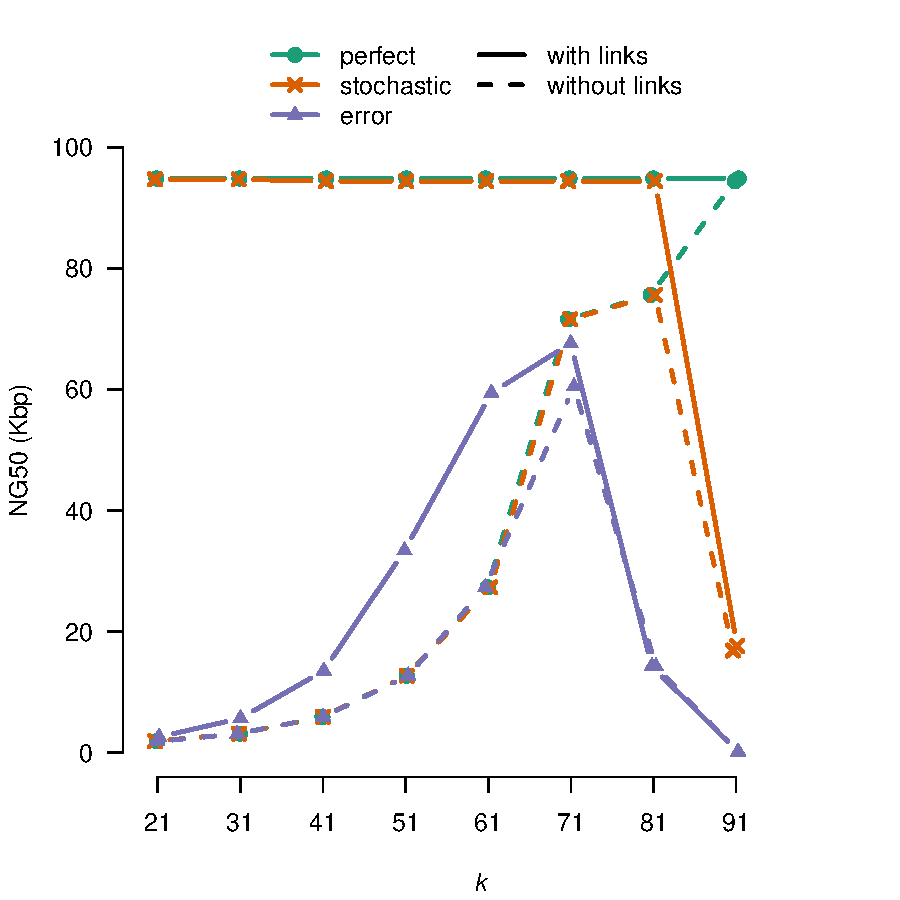
\includegraphics[width=1\linewidth]{../plain-vs-links.pdf}
\caption{SE reads}
\end{subfigure}
\begin{subfigure}{.45\textwidth}
\centering
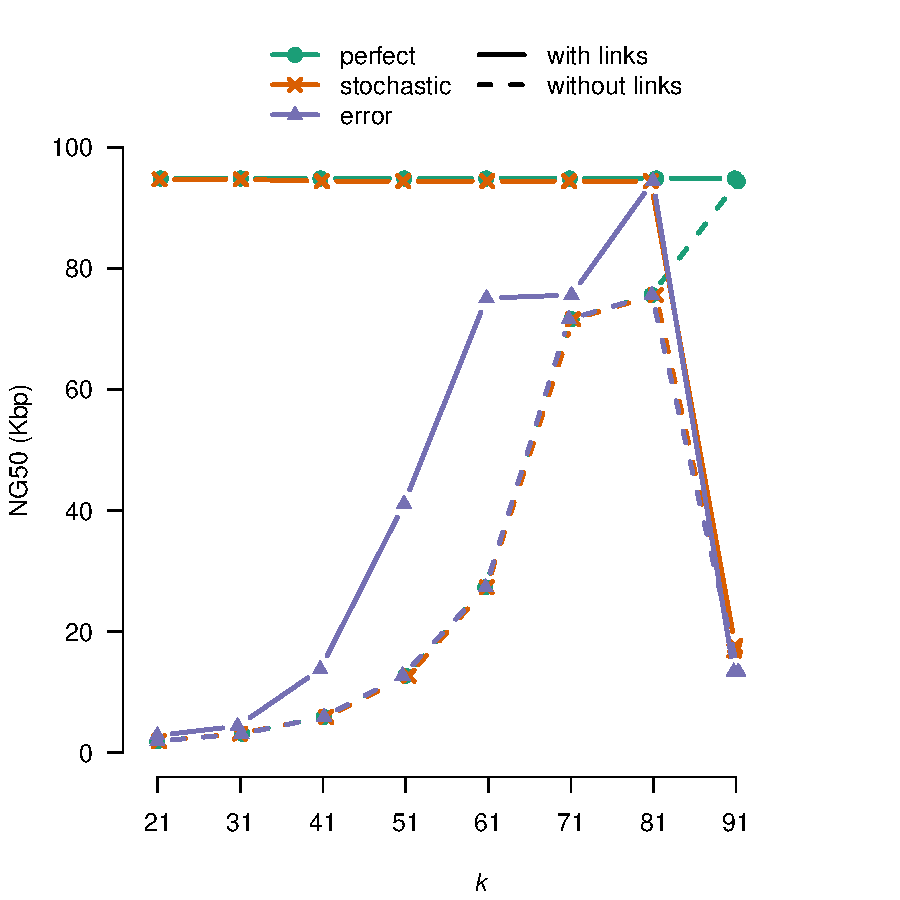
\includegraphics[width=1\linewidth]{../plain-vs-links-corr.pdf}
\caption{SE reads + \texttt{bfc} error correction on ``error'' reads}
\end{subfigure}
\begin{subfigure}{.45\textwidth}
\centering
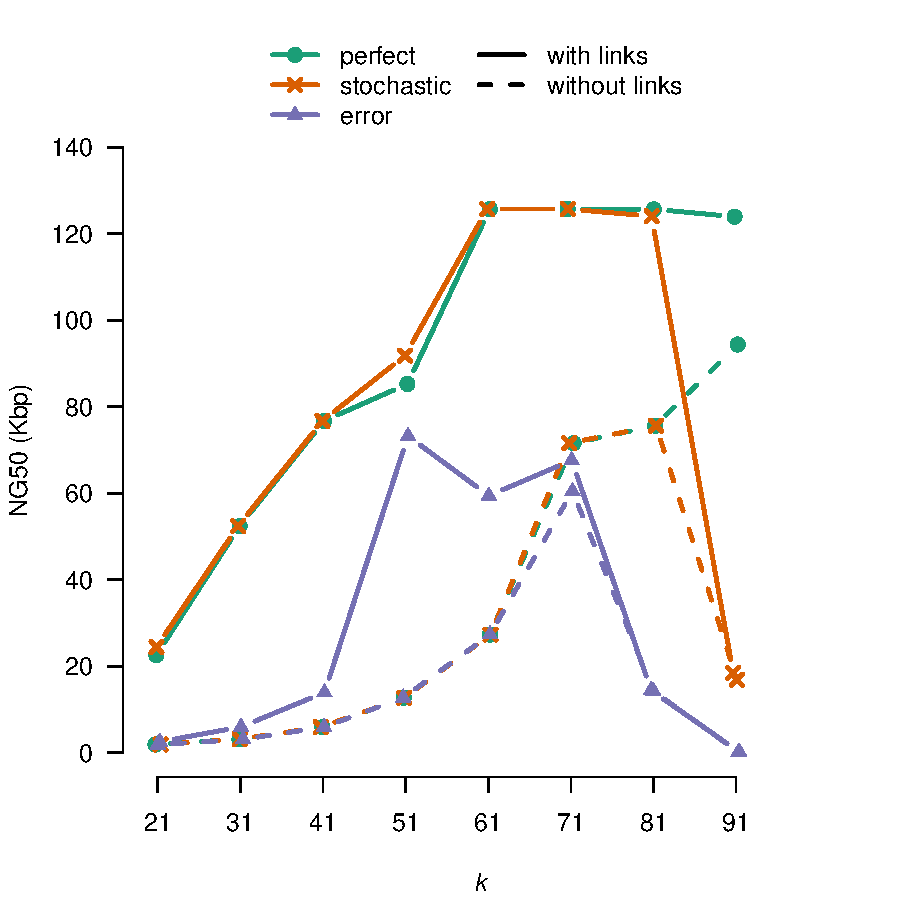
\includegraphics[width=1\linewidth]{../plain-vs-pe.pdf}
\caption{PE reads}
\end{subfigure}
\begin{subfigure}{.45\textwidth}
\centering
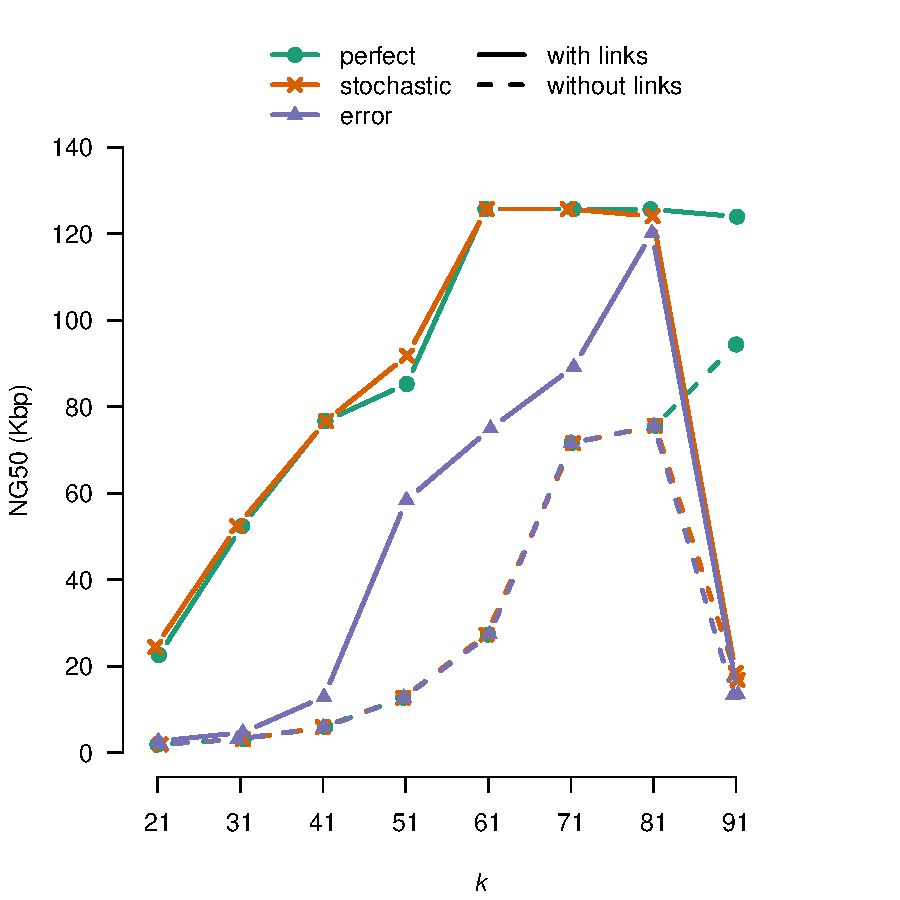
\includegraphics[width=1\linewidth]{../plain-vs-pe-corr.pdf}
\caption{PE reads + \texttt{bfc} error correction on ``error'' reads}
\end{subfigure}
\caption{Assembly length metric NG50, on raw de Bruijn graphs (i.e. without links, dashed lines) and linked de Bruijn graphs (i.e. with links, solid lines), as a function of \kmer{} size. Assembling $1$ Mbp of sequence (human GRCh37 chr22:28,000,000-28,999,999) with three simulated 100X read data sets: (i) error free $100$ bp reads, one read starting at every base (``perfect''); (ii) error free stochastic coverage, uniformly distributed read starts (``stochastic''); (iii) an error rate of $0.5\%$ and stochastic uniformly distributed coverage (``error''). Top row: SE reads. Bottom row: PE reads. Left column: no third party error correction; right column: \texttt{bfc} run on ``error'' reads data set.}
\label{fig:ng50sim}
\end{figure}

% SGA
\begin{figure}[H]
\centering
\begin{subfigure}{.45\textwidth}
\centering
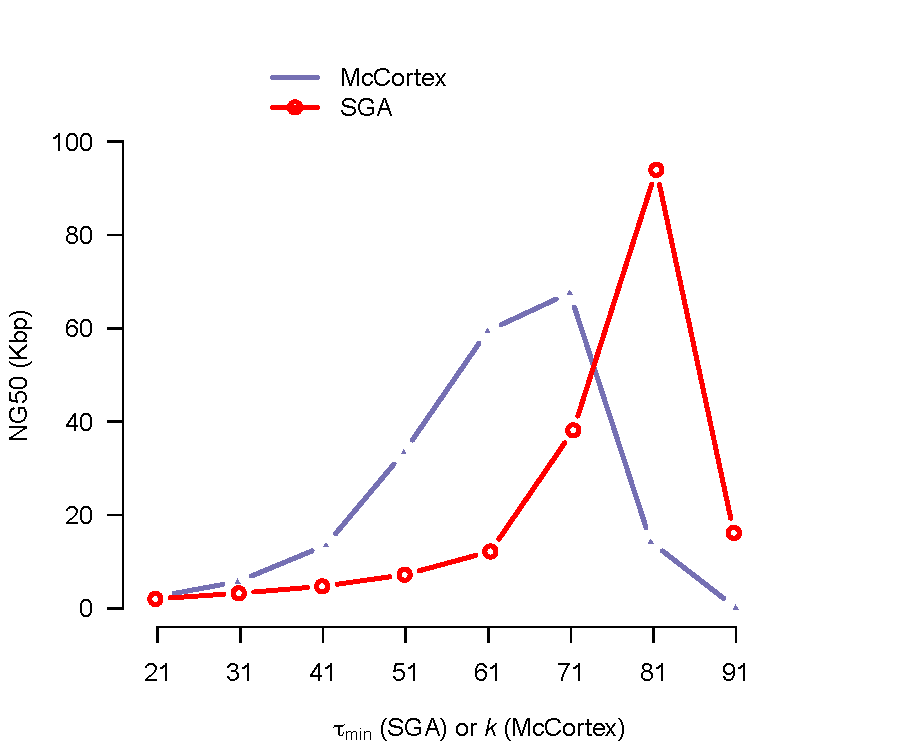
\includegraphics[width=1\linewidth]{../links-vs-sga-ng50.pdf}
\end{subfigure}
\begin{subfigure}{.45\textwidth}
\centering
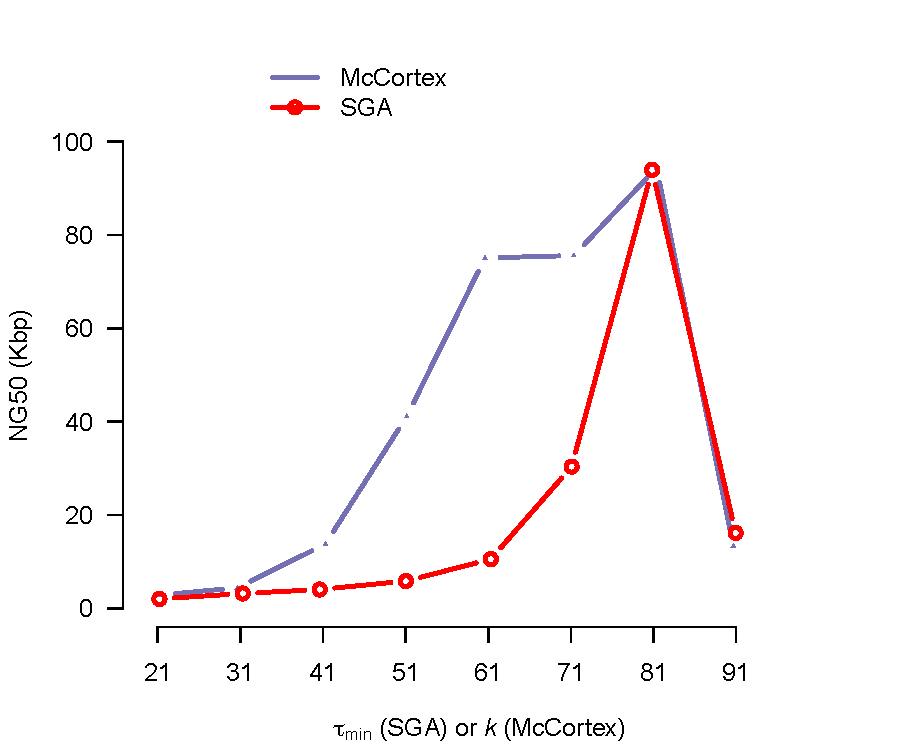
\includegraphics[width=1\linewidth]{../corr-links-vs-sga-ng50.pdf}
\end{subfigure}
\begin{subfigure}{.45\textwidth}
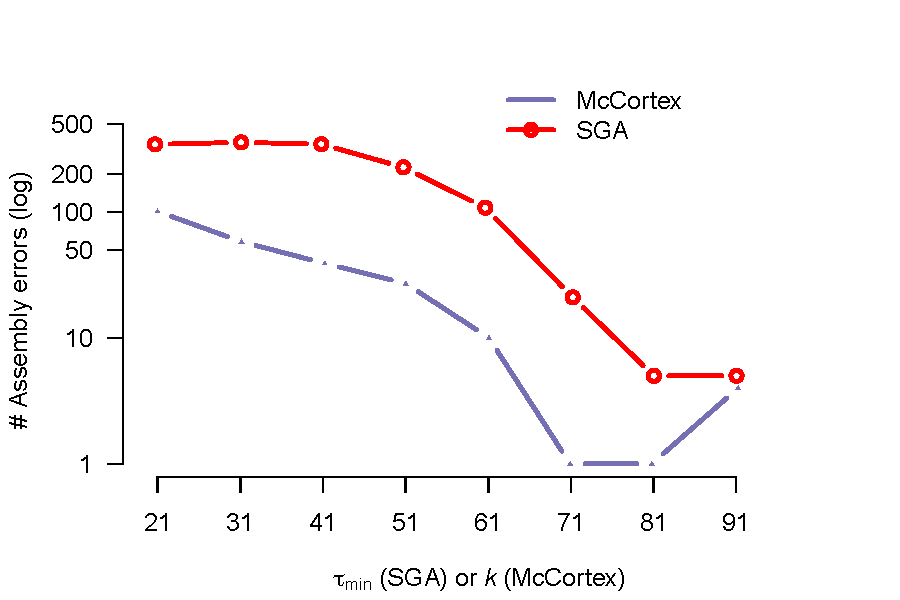
\includegraphics[width=1\linewidth]{../links-vs-sga-errs.pdf}
\caption{SE reads}
\end{subfigure}
\begin{subfigure}{.45\textwidth}
\centering
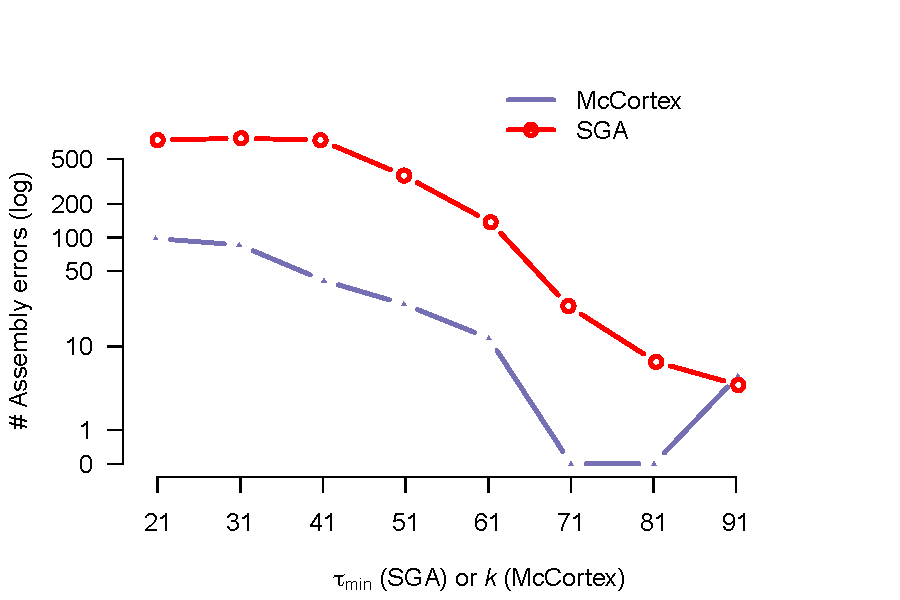
\includegraphics[width=1\linewidth]{../corr-links-vs-sga-errs.pdf}
\caption{SE reads; Using \texttt{bfc} error correction on ``error'' reads}
\end{subfigure}
\caption{Assembly results for \texttt{SGA} and \texttt{McCortex} compared using a simulation on $1$ Mbp of sequence (human GRCh37 chr22:28,000,000-28,999,999), using $100$ bp reads with an error rate of $0.5\%$ and stochastic 100X coverage (``error'' data set from Figure \ref{fig:ng50sim}). Top row: contig NG50 at different parameters of $\tau_{min}$ (\texttt{SGA}) and $k$ (LdBG). Bottom row: number of assembly errors in contigs compared to truth. Left column: no third party error correction. Rigtht column: using \texttt{bfc} error correction before assembling}
\label{fig:sga-vs-mccortex}
\end{figure}

\end{document}
